%
% DSP Report Template
%
% (c) 2005 EMT DSP Group
%
\documentclass[12pt,a4paper]{article}
%\usepackage{dsp_report}

\usepackage{parskip}

% randausgleich bei kleinen zeichen mit wenig deckung rechts
% % http://latex.tugraz.at/latex/fortgeschrittene#optischer_randausgleich
\usepackage[activate=normal]{pdfcprot}


%
%\DSPTitle{Odometry for Wheeled Mobile Robots}
%{Michael Maier}

\usepackage{graphicx}

\usepackage{subfigure}
\usepackage{xspace}                   % space nach makro
\usepackage[left]{eurosym}            % Euro symbol
\usepackage{hyperref}

\newcommand{\mbnote}[1]{\textcolor{Gray}{\textbf{\noindent M. Brandner NOTE: #1}}}
\newcommand{\mmnote}[1]{\textcolor{Gray}{\textbf{\noindent M. Maier NOTE: #1}}}
\newcommand{\MH}{\emph{``Mostly Harmless''} RoboCup Team\xspace}
\newcommand{\MSL}{Middle Size League\xspace}
\newcommand{\robocup}{\emph{RoboCup}\xspace}

\begin{document}

%% Based on a TeXnicCenter-Template by Tino Weinkauf.
%%%%%%%%%%%%%%%%%%%%%%%%%%%%%%%%%%%%%%%%%%%%%%%%%%%%%%%%%%%%%

%%%%%%%%%%%%%%%%%%%%%%%%%%%%%%%%%%%%%%%%%%%%%%%%%%%%%%%%%%%%%
%% Deckblatt
%%%%%%%%%%%%%%%%%%%%%%%%%%%%%%%%%%%%%%%%%%%%%%%%%%%%%%%%%%%%%
%%
%% ATTENTION: You need a main file to use this one here.
%%            Use the command "\input{filename}" in your
%%            main file to include this file.
%%
\begin{titlepage}

  \begin{center}
    \begin{minipage}[htb]{18cm}
      \hspace*{-2.6cm}
      \includegraphics[width=3.3cm]{./figures/logos/EMT.jpg}
      \begin{tabular}{p{10cm}}\centering{
      \Large Institute of Electrical Measurement and Measurement Signal Processing\\ Graz University of Technology
      ~\\
      ~\\}
      \end{tabular}
      \includegraphics[width=3.3cm]{./figures/logos/TUG.jpg}
    \end{minipage}

    \Large {Bachelor's Thesis\\} %
    \vspace*{1cm} \huge{\textbf{Odometry for Wheeled Mobile Robots}\\}
    %
    \vspace*{1.0cm} 
    %\Huge{\textbf{#1}\\}\vspace*{2.5cm} \vfill
    \Large{Michael Maier\\} \vspace*{1cm}
    %
    \Large{Supervisor: Dipl.-Ing. Dr. Markus Brandner\\} \vspace*{0.5cm}%


    \begin{minipage}[htb]{18cm}
      \hspace*{-0.4cm}
      \includegraphics[width=3cm]{./figures/logos/MH.jpg}
      \begin{tabular}{p{10cm}}\centering{
        \Large Mostly Harmless RoboCup Team \\Institute for Software Technology, \\Graz University of Technology\\
        \texttt{team@robocup.tugraz.at}\\ \texttt{http://www.robocup.tugraz.at}
        ~\\
        ~\\}
      \end{tabular}
    \end{minipage}

    \Large{Graz, \today}

  \end{center}
\end{titlepage}


\tableofcontents
\clearpage
\pagestyle{plain}


\begin{abstract}
Abstract

% 1p
\end{abstract}

\clearpage

\section{Introduction}


\subsection{RoboCup}

The RoboCup is an international research and education initiative. 
It's goal is ``By the year 2050, develop a team of fully autonomous robots that can win against the current human soccer world champion team"~\cite{robocup.org}.
It encourages research in the field of robotics, e.g.\ machine vision, machine learning, autonomous systems.

%|| to Apollo Program.

Every year, a world championship is held accomplished by a conference in a different city around the globe.
Also, various local competitions and conferences are held by local groups.

The RoboCup is divided into three parts: RoboCup Soccer, Rescue and @Home.
Every division is divided into several leagues targeted at different challenges.

%1/2 page

\subsection{\MSL}

In RoboCup Soccer, the \MSL is the most challenging.
The robots have to be fully autonomous.
All sensors, actuators and computation are on board, no external input is allowed.
A Team consists of at most 6~robots with a size of max. $50\times50\times80$\,cm$^3$.

The game is played on a field of $12\times18$\,m$^2$ and lasts $2\times15$~minutes.
The game field surface is usually carpet.
The \MSL is the only league, where an official FIFA ball is used.
Objects are distinguished by colour, the game field is green with white lines, robots and referees are black and the ball is red.

The rules are official FIFA rules~\cite{msl-rules} with slight adaptations for robotic players.
The game rules are tightened every year to keep up with the technological progress. 
E.g. the field size has grown from $6\times8$\,m$^2$ to $12\times18$\,m$^2$ since introduction of the \MSL.

More than 20 teams from all over the world participate in the \MSL, almost all with academical background.

% 1/2 p

\subsection{\MH}

The \MH participates in the \MSL. 
It's name is a reference to the ``Hitchhiker's Guide to the Galaxy'' by Douglas Adams~\cite{h2g2}.
It was founded 2003 at Graz University of Technology at the Institute for Software Technology. 
It consists solely of students and acts as a platform for master's, bachelor's thesis and seminar projects.
Currently, more than 30~students are working on the robots in their free time.

It regularly participates at European championships as well as World Championships.
RoboCup 2009 in Graz was the first time the team advanced a round in a World Championship. 
Also, the third place in the technical challenge was won.



% 1/4 p

\subsection{Current Robot Platform: Krikkit}

The ``Krikkit'' robot platform was built in 2006~\cite{}. 
It was designed solely for playing soccer, in contrast to the old, multi-purpose research robot platform.
Nearly all components, from electronics to mechanical parts are developed in-house.
Four robots were built and made their début at the World Championship 2006 in Bremen.

Some of the main features of the ``Krikkit'' robot are shown in \autoref{fig:krikkit}.

\begin{figure}[ht]
\begin{center}
\includegraphics[width=0.5\columnwidth]{figures/krikkit.pdf}
\caption{\label{fig:krikkit}
Krikkit robot. Omni-vision with camera and mirror~(1); Industrial PC~(2); Pneumatic kicker~(3); Omni-drive is below the black bumper.
}
\end{center}
\end{figure}

It has a $360^\circ$ omnidirectional vision system via a firewire-camera pointing upwards to a hyperbolic mirror.\\
Its brain is a standard mini-ITX industrial PC.\\
A powerful pneumatic kicker with a~200\,bar pressurised air bottle as supply enables the robot to kick the ball approx. 10\,m forward.
The kicks are such powerful, that the vibrations destroyed the former-used hard disks, now replaced with SSD~storage.
Also, every kick caused a camera blackout of nearly 2~seconds due to the vibrations.\\
Its drive system is also omnidirectional and is based on self-designed Mecanum wheels~\cite{mecanum2007}. 
The $45^\circ$-Arrangement of the wheels (see~\autoref{fig:mec-wheel}) promised smooth and vibration-free operation.
The three wheels are arranged in $120^\circ$-steps (see~\autoref{fig:omnidrive}) and are driven by a 200\,W brushless DC motor for each axis.
Due to the nature of omni-wheels, the robots are able to move in any direction and any orientation.\\
The motors and all other electric components are supplied by a smart battery system~\cite{krammer06} with NiMH rechargeable batteries.
All electronic components are connected via CAN-Bus.

\begin{figure}[hb]
  \begin{minipage}{0.45\textwidth}
   \centering
    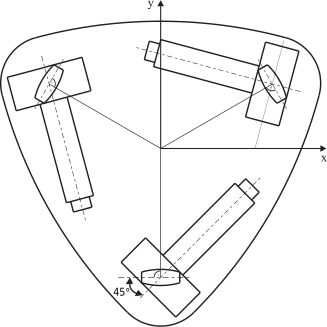
\includegraphics[width=1\textwidth]{figures/krikkit_drive_angles}
    \caption{\label{fig:omnidrive}Omni-drive schema of the Krikkit robot. Three $45^\circ$ Mecanum wheels have their small wheels arranged in a circle around the centre.
    \cite{mecanum2007}}
  \end{minipage}\hfill
  \begin{minipage}{0.45\textwidth}
   \centering
    \includegraphics[width=1\textwidth]{figures/Omniwheel_drive.png}
    \caption{\label{fig:mec-wheel}Mecanum wheel with motor and gearbox.}
  \end{minipage}
\end{figure}


The Krikkit robots served well for four years, much was learned.
Before RoboCup~2009 in Graz, a major mechanics overhaul was done.
In the meantime, all major electronic components also reached the end of their life cycle.
With the knowledge gained, lost and acquired again the successor of the Krikkit generation is in development now.
    

\subsection{In Development: Krikkit3G}

The next generation of robots is in development since mid-2010.
It will be a direct successor of the Krikkit generation, therefore the name \emph{Krikkit3G}.
The successful concepts are are adopted nearly unchanged:

\begin{itemize}
  \item omnidirectional drive with the three Mecanum Wheels
  \item the omni-vision system
  \item pneumatic kicking concept
  \item the use of a standard mini-ITX industrial PC
  \item modularity of all components
\end{itemize}

The new robot design focuses on the strict modularity of all components.
It has been shown that fast disassembling and replacing of critical components is crucial in the fast-paced tournament environment.
Especially the power train has been modularised, the wheel, gearing, motor and motor electronics can be swapped as a whole group.

Tests showed that the smoothness of the Mecanum wheels was insufficient due to manufacturing imprecision.
The resulting vibrations should be filtered out by an independent wheel suspension.

%  bumpers ?

For the kicking system, the pneumatic principle was kept.
But it is now much more versatile. 
It can switch between high and flat kicks at full power, and side-kicks are also possible now.
It features a new ball guidance system, which allows grabbing the ball for a short moment.
This becomes especially useful when decelerating.
Also, the vibrations from the kicker disturbing the camera should be reduced by an active final position dampening system.
Nevertheless, short disturbances in the vision system due to the vibrations will remain during the kicks.

Big changes were made in the electronics sector.
A new microcontroller core (An ARM Cortex~M3) is used on every component, replacing the different microcontroller architectures used before.
The smart battery system also got a major upgrade, featuring even smarter batteries.

In the mechanical design, space is now also provided for an improved odometry system, which will be developed based on this work.


\begin{figure}[b]
\begin{center}  
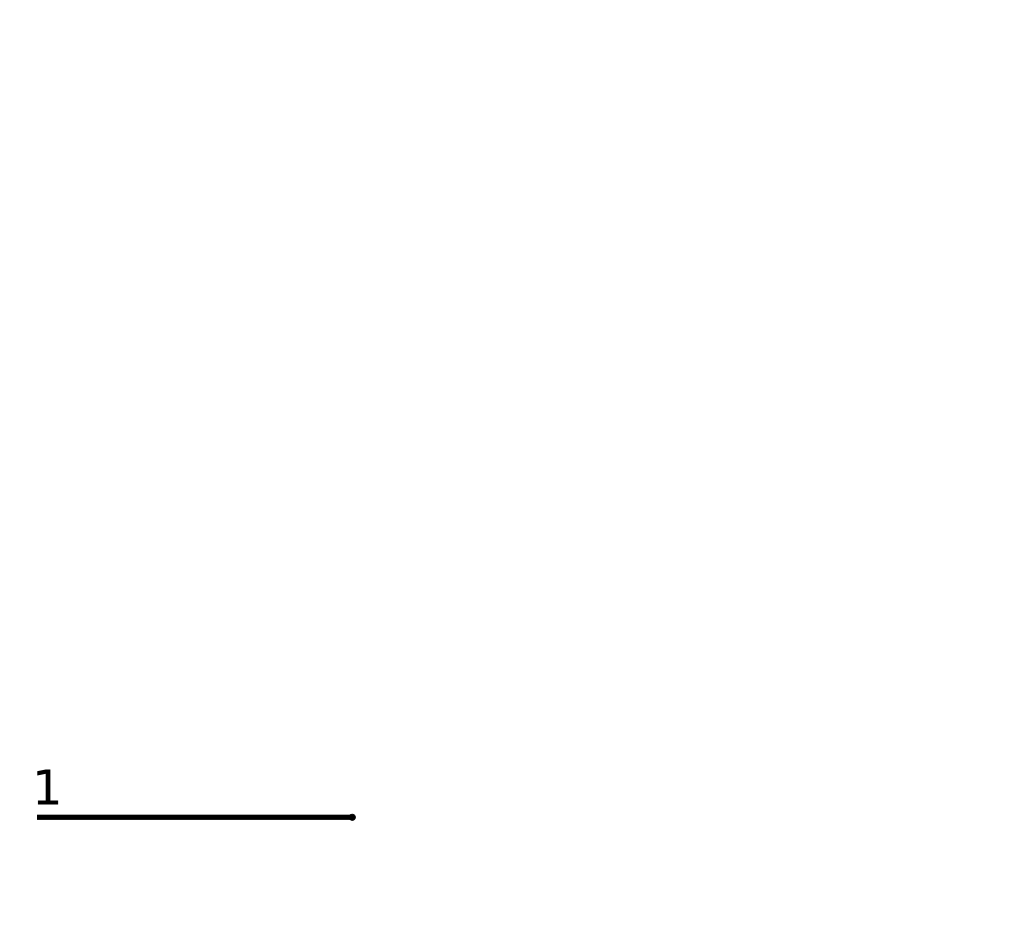
\includegraphics[width=0.5\columnwidth]{figures/Krikkit3G.jpg}
\caption{\label{fig:krikkit3g}
Rendering of the Krikkit3G robot (Without outer hull).
}   
\end{center}
\end{figure}


% 1p

\subsection{Odometry}

%  Definition
%  Verwendungsmoeglichkeit
%    Lokalisierung
%      higher framerate than cam
%      backup-system for cam
%    Motion control
%      anti-slip regulation

Odometry, better known as path measurement is important for every moving vehicle, especially robots which need to know where they currently are. 
The best known odometry measuring is used in cars as kilometre reading on the tachometer.

For autonomous mobile robots, odometry plays an even more important role.
Together with the vision system and the compass, it is a part in the sensor fusion for building the world model.
In the current Krikkit software, is is used for the following purposes:
At first, it acts as an initialisation vector for the vision system, when comparing two camera frames for calculating the offset between them.
The second important role comes from the high frequency odometry data is available.
Odometry data is provided with a frequency of 50\,Hz. 
This is much faster than the currently used vision system (15~-~25\,Hz). 
Therefore its values are added to the last known position in the world model for the time between two camera frames.
At last, it acts as a backup system for the mainly vision based localisation system in case of camera blackouts, e.g.\ blurred images due to the vibrations from a kick or a collision.

There are more possible use cases for odometry not implemented yet, e.g.\ anti-slip regulation for every single wheel.



\subsection{Motivation for this Work}
  
Current odometry systems of the Krikkit generation is based on the rotational speed of the wheels.
This has the major disadvantage of the accuracy bound to the slip of the wheels.
The problem is the non-uniform structure of the game field carpet, which has different slip factors in each direction.
Due to the different speeds and angles of the Mecanum wheels, this leads to deviations even when driving a straight line.
The errors accumulate over time, resulting in $90^\circ$~deviation on 10\,m straight distance driven.

Therefore, an wheel-independent odometry system has to be developed.
The goal of this work was:

\begin{itemize}
  \item Gathering requirements for a sensor
  \item Search for different types of sensors
  \item Implementation and validation of a prototype
\end{itemize}


\subsection{Requirements for a new type of Odometry Sensor on the Krikkit/3G platform}

The \MSL provides an ideal testbed for mobile robotics.
The main demands in robotics are miniaturisation, low cost and energy usage, and robustness to the environment.

The range of application in the \MSL demands the following design parametersa for an odometry sensor:
\begin{itemize}
  \item must deliver linear and rotational accurate data in three degrees of freedom
  \item must work on green carpet, other surfaces are bonus.
  \item must not emit radiation or other disturbing effects irritating other robots or humans
  \item resistance against dust from the carpet abrasion
  \item shock resistant
\end{itemize}

The carpet is a particularly hairy concern, as its choice is up to the event organizer.
The only restriction in the \MSL rules and regulations~\cite{msl-rules} is: green.
Therefore, the game field surfaces differ in colour and surface roughness on every event.
Colours from bright green over dark teal to nearly grey have been seen over the past years.
The roughness is another chapter, it ranged from a very even felt with a roughness with a maximum of 2\,mm to an artificial grass like carpet with 15\,mm long hairs. 
Depending on the carpet the robot sinks in some millimetres, which also affects the clearance height.

The \MH requirements for a new odometry sensor are speeds of at least 5\,m/s at an operating frequency of at least 50\,Hz.
From the software side, it would be highly appreciated if the sensor would deliver data quality information.
Data quality information is crucial for the sensor fusion to recognize and de-prioritize erroneous data.
The \MH had bad memories about a malfunctioning compass ruining the world model.
At last, the \MH has very tight budgetary limitations, due to being a students-only team depending on external sponsors.
The sensors have to be cheap enough to be affordable for series for up to six robots.


On the Krikkit3G robots, the available space is limited to $50\times50\times110$\,mm for each of the three proposed sensor mount points.
The Krikkit3G robot, similar to the old Krikkit generation, has a clearance height of 20\,mm.
Due to the new independent wheel suspension, the operating range of the sensor must be greater than $\pm 5$\,mm to the reference plane.
Data must be output on the robot's CAN-Bus.
As power supply only two DC lines with 24\,V and 7\,V are available at reasonable currents.





\clearpage
\section{State of the Art in Odometry Measurement}

When determining the position or movement of a vehicle, one has the following choices: 
Relying on global or relative position measurement.

The best known global position measurement is the Global Positioning System GPS.
This is widely used in robotics in outdoor applications, where a GPS signal is available.
Indoors, other known landmarks can be used.
In RoboCup, the well-known shape of the soccer field is used for global reference.
Without exception, every soccer robot uses the features of the game field, e.g.\ the goals, lines and corner posts for orientation.\\
Other global approaches for gathering position data are compasses and gyroscopes.
They also deliver global data, but orientation and not positioning. 
This approach delivers only one of the three degrees of freedom needed, but it can complete the missing dimension.

% - global positioning
%   GPS
%   Compass
%   gyroscopes
%   relative position to known landmarks
%   - poles from 2006
%   - lines on the game field

For relative position measurement, one has the choice to measure distance, velocity or acceleration.
Every approach has its advantages, depending on the use case.
When aiming for the distance travelled, it is not wise to measure acceleration, hence the measurement errors would sum up quickly due to the twice integration.\\
When measuring acceleration, one has the choice between industrial grade accelerometers as used e.g.\ in aeroplanes, and consumer grade accelerometers based on the piezoelectric effect.\\
Speedometers exist in various implementations based on the Doppler effect, e.g.\ radar.\\
Distance meters can be mechanical or optical.
The simplest mechanical distance meter is a measuring tape.
Or when used on moving vessel, the log-line of a sailing ship used for speed measurement.
In the last decade, another electronic approach was developed: optical distance meters based on comparing images for translational displacement, as used in optical computer mice.

% - relative positioning
%   - acceleration
%   - velocity
%   - distance
%   accelerometers
%   speedometers relying on the Doppler-effect
%   mechanical distance meters (like in cars or early computer mice)
%   optical distance meters based on comparing images for translational displacement, as used in optical computer mice


Every approach has properties to evaluate:
\begin{itemize}
  \item maximum and minimum speed capability
  \item maximum and minimum acceleration
  \item number of dimensions of movement data one sensor delivers
  \item linearity and deviation of data
  \item length of time of a single measurement
  \item lag between measurement and data availability
  \item highest possible frequency of measurements
  \item resilience against reference surface distance changes
  \item maximum and minimum distance to reference surface
  \item surface state requirements
  \item resilience against environmental changes
  \item influence of the sensor to the environment 
  \item size and power requirements of the sensor
  \item cost of the sensors for three dimensions
\end{itemize}

In preparation for this work, a lot of sensor types, both industrial and consumer grade, were evaluated for the use in the \MSL based on these properties.


\subsection{Possible Odometry Sensors Types}



\subsubsection{Accelerometers}

An accelerometer consists mainly of flexible mounted mass that is under the influence of a force.
If the mounting consists of springs, the displacement is linear to the applied force.
This displacement is then measured.
Under normal circumstances on earth, every object is under the influence of the gravitational force.
Therefore, 1\,g must be subtracted from the result.

In commercial sensors, piezoelectric elements are used to convert the force into a signal.
In the last years, the use of micro electro-mechanical systems (MEMS) has been increased significantly.
Sensors for three dimensions are available now in tiny package formats at low cost for consumer applications.

\subsubsection{Gyroscopes}

A gyroscope is an inertial sensor, that detects the change of position.
Historically, they were flywheels mounted in a Cardan suspension. 
Based on the principles of conservation of angular momentum, when spin up they remain at their orientation.

Today they are implemented as MEMS similar to accelerometers mentioned.
Often they are even combined with accelerometers in a single chip package to 6-dimensional sensors.


\subsubsection{Ultrasonic Doppler Velocimetry}

Ultrasonic Doppler velocimeters  work similar to ultrasonic distance sensors.
The main use today is in liquid flow  measurements.


\subsubsection{Microwave Doppler Velocimetry (Radar)}

Radar is an umbrella term for object detection systems utilizing electromagnetic waves from 300\,MHz up to 3\,THz~\cite{nrt}.
It can be used to measure the distance of objects and also their speed through the Doppler effect.
Depending on the object distance, different wavelength are used.
For short-range measurements, e.g.\ radar guns, and also for speed measurements on moving vehicles itself, short-range microwave sensors with 24\,GHz are used.~\cite{s_r_radar}

\subsubsection{Laser interferometry}

Speed measurement with laser interferometry is divided into two approaches, one called Laser Doppler Velocimetry and the other is referred as Laser Doppler Vibrometry.\\
Two coherent laser sources are intersected on the moving target surface at different angles.
The interference of the two beams creates a set of straight fringes. 
Particles of the surface moving thorough the fringes reflect light on the constructive interference.
The resulting frequency is then captured by a photo diode.

% source: WP

- vibrometer
  beam is split into two coherent, one is reflected and interfered with the original beam, which is collected in a photo diode. 
  the frequency shift between the two results in a beat at the detector.

% source: WP

\subsubsection{One-dimensional Optical Spatial Frequency Filtration}
1/4
\subsubsection{Industrial/Custom-build Optical Speed Sensor}
        Daniel's approach~\cite{Hrach2006}
        laser speckle applications (Dehnungsmessung) 
1/4
\subsubsection{Optical Mice}
1/2

\subsection{Current Implementations used in RoboCup}

\subsubsection{\MH}
      wheel encoder
        probleme
\subsubsection{Other Teams}
      2. satz raeder
        probleme

  accelerometers -> only nao for inertial informations, not for navigation

\subsection{Decision for a Type of Sensor}

The focus lies on cheap consumer-grade sensor based solutions, due to the hefty price for industrial sensors.

  entscheidung fuer einen Sensortyp
    - why/why not...
    - ...
    - ...
        2G spitzenvibration -> no


\section{Sensor Design}

block diagram
  ADNS + optic
  XC
  PC

\subsection{Optical System}
  requirements

micro-bench system

Sketch

\subsubsection{Optical Path calculations: Original Mouse Setup}

\subsubsection{Optical Path calculations: 2-Lens Setup}

\subsubsection{Optical Path calculations: Telecentric Setup}


\subsubsection{Sensor mounting \& Calibration}

Sketch with adjusting screws in all dimensions

calibration process
  laser

\subsubsection{Lens 2 \& Aperture Mounting}

manufacturing drawing

\subsubsection{Illumination}

  Why here?
  types of LEDs and Lasers used
 
  Illumination PCB

  circuit

  PCB print


\subsection{Electrical Design}

\subsubsection{The ADNS 6010}

specs

workflow diagram (from datasheet)

ADNS-testplatine
  requirements

  circuit diagram

  PCB drawing

\subsubsection{The XC164CM Microcontroller}

Specs etc

XC-164 eval board 
  Image from datasheet

Wiring of the Evaluation Board

  block diagram

  circuit

\subsection{Software}

\subsubsection{uC - Software}

  XC-Code
    requirements
    firmware catch

    image streaming

    motion data streaming
      + reference sensor

\subsubsection{PyQT GUI}

\subsubsection{Octave Analysis Scripts}

\section{Experimental Setup}

- requirements

\subsection{Mechanical Design of the Testbed}

block diagram

\subsection{Motor \& Disk}

\subsection{Reference Speed Sensor}
      Picture of sensor from Datasheet
      electrical setup used

\subsection{Microcontroller \& Host PC}      

\section{Experimental results}

\subsection{Illumination tests}

\begin{itemize}
  \item Laser
  \item Studio Spotlight
  \item ultra-bright white LEDs
  \item IR-LEDs
\end{itemize}

\subsection{Non-telecentric tests}

\subsection{Telecentric tests}

\subsubsection{Carpet 1}

\subsubsection{Carpet 2}

\subsubsection{Carpet 3}

\subsubsection{Game Field Lines}

\subsection{Interpretation}

  plots
  ergebnisse

\section{Conclusions \& Outlook}

  evaluation of a combination of IR-LED illumination and Laser illumination

  newer sensor ADNS-90xx

  mechanical limitations
    size constraints
    dirt cleaning...
  electrical requirements
    new architecture: ARM
    also include illumination control in uC
      use of the shuttered illumination for higher power 
      use of both LEDs and Lasers for white lines
  software algorithms: compute 3 dimension out of 2/4/6

ca 3-5p


summe gesamt 49 Seiten (ohne abstract, inhaltsv, bibl.)


%--------------------------------------------------------%
% Bibliography
%--------------------------------------------------------%
\addcontentsline{toc}{section}{Bibliography}
\label{Bibliography}
\bibliographystyle{plain}
\bibliography{literature}
%
\end{document}

% vim: spell spelllang=en_gb:
